\section{Context}

This research is the latest on a long line of academic articles on retrieval-augmented generation, comparing and contrasting parametric knowledge with contextual information, and how to enhance knowledge on large language models.

This section summarizes key articles that informed this research.

\subsection{Foundational Papers on Large Language Models}

Large language models have exploded in popularity since the development of transformer architecture \citep{attention_is_all_you_need}.
This architecture relies entirely on self-attention mechanisms rather than recurrent layers, which allow the model to weigh the importance of different words in a sequence relative to each other, irrespective of their position.
This mechanism enables the model to capture complex dependencies and relationships across long sequences more effectively than traditional models.

\begin{figure}[htb]
	\centering
	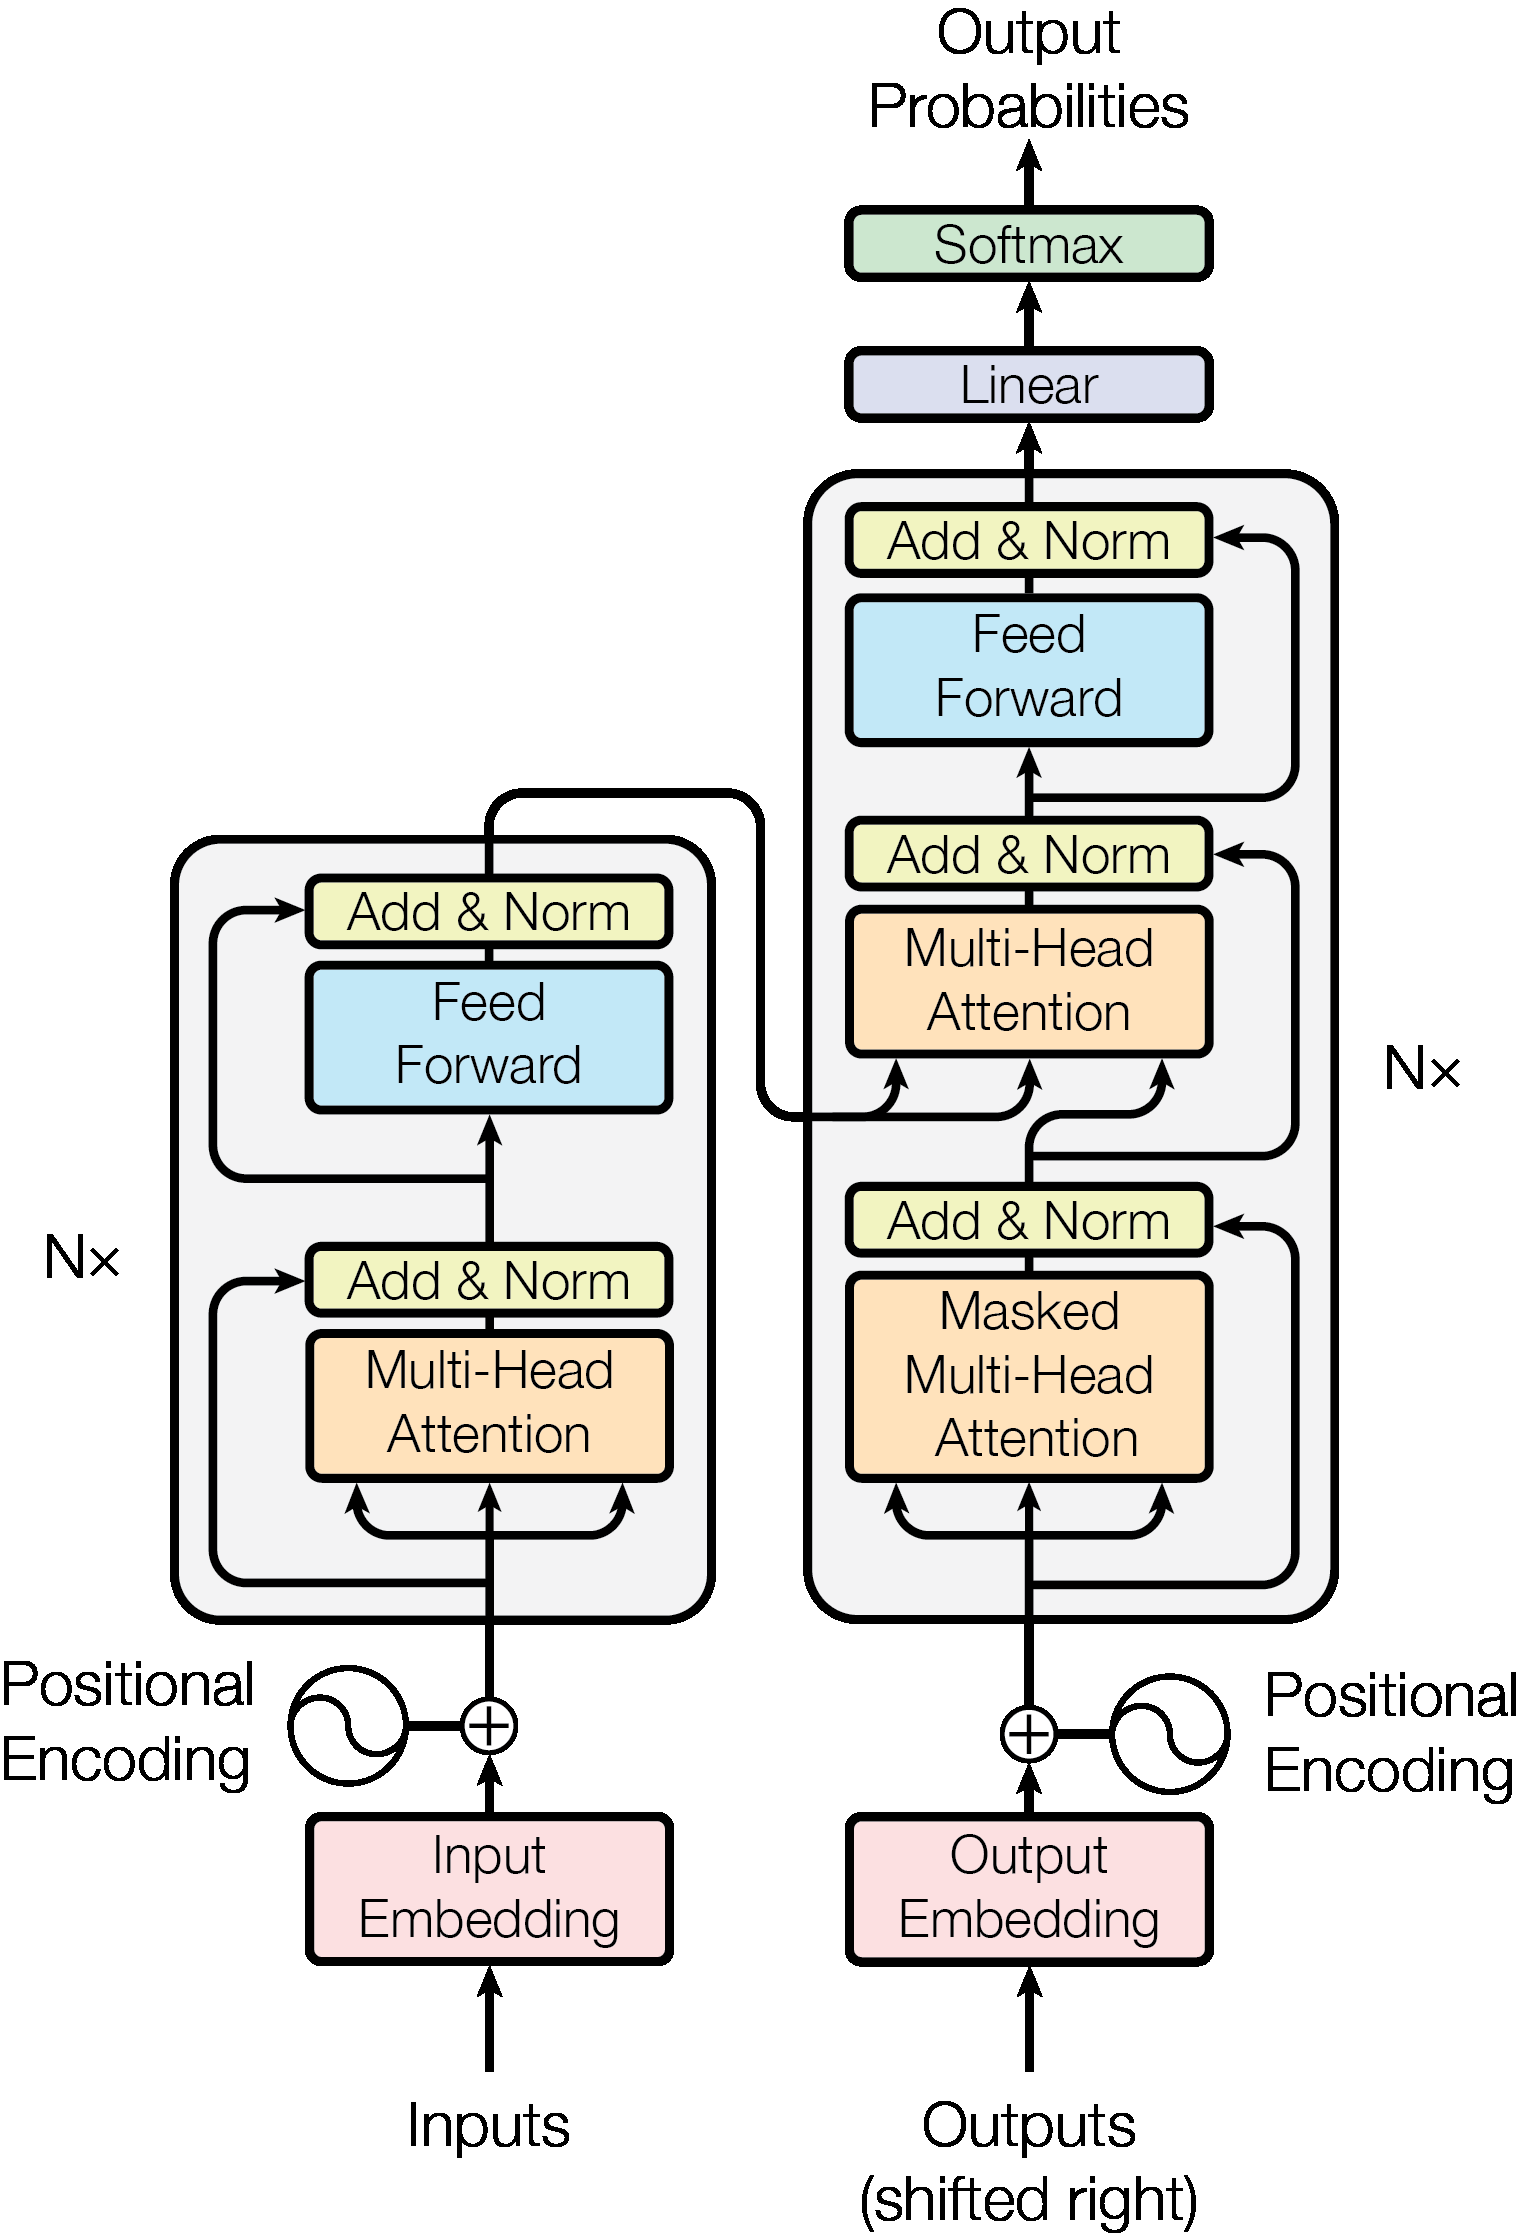
\includegraphics[width=.37\textwidth]{transformers.png}
	\caption{Transformer Architecture, from ``Attention is all you need'' \citep{attention_is_all_you_need}.}
\end{figure}

GPT models \citep{gpt} improve upon this architecture by running a supervised task-specific fine-tuning round after the unsupervised pre-training on large amount of test data.
Later models, starting from GPT-2, use zero-shot transfer learning to improve their performance \citep{gpt2}.
Zero-shot learning \citep{zeroshotlearning} trains a model to perform a task without having been explicitly trained on examples of that task; instead, it leverages knowledge gained from pre-training to infer and generalise to new tasks with the context on the prompt.

By adding only a few examples of the task at hand, a model can improve generalisation to new tasks with a limited amount of labelled data.
GPT-3 uses this to understand the structure and nature of a task with a few examples \citep{gpt3}.

Despite these improvements in sequential models, the models still present many faults in question-and-answer tasks \citep{how_can_we_know}.
Hallucinations are not uncommon, even for queries that ask questions that can be answered with short answers.

\subsection{Architectures of Large Language Models}
\label{llm_architectures}

In this subsection we present two different large language model architectures that are used widely for this research.
This thesis uses and compares four models using the Flan-T5 and Llama architectures.

\subsubsection{Seq2Seq Models: T5 and Flan-T5}

The T5 model \citep{t5}, developed by Google Brain in 2020, is an encoder-decoder Seq2Seq model that treats every processing problem as a text-to-text task.
This way it uses transfer learning to learn many different kinds of tasks from a single source of training data.

The model is trained using only masked language modelling and treating every problem as a supervised text-to-text task where both the input and output are in text form.
The data is later fine-tuned to make it able to solve other tasks.

\texttt{Flan-T5} uses the same architecture as T5, but fine-tuned on tasks to follow explicit instructions \citep{flant5}.
This scales well on larger tasks and larger model sizes, and it's particularly effective on problems requiring a chain-of-thought.

These models have strong performance while adding little or not existing context, and are capable capable to understand explicit instructions which can generalise to new task types, improving the downstream task performance \citep{flan_performance}.

\subsubsection{Decoder-only Models: GPT and Llama}

GPT models use a transformer-based decoder-only architecture trained to solve the problem of causal language modelling, or predicting the next token in a sequence \citep{gpt,gpt2,gpt3}.
These models generate text by predicting tokens one-by-one rather than encoding internal information of a query, such as Seq2Seq models.

GPT models are good at solving a variety of tasks they they not trained in with little or no context.
Its autoregressive nature specialised it at generating human-like text, so it's widely used for chatbots and content creation.

Llama models improve several limitations of GPT by training smaller models on more data \citep{llama}, which generally achieves better performance \citep{hoffmanetal}, and various improvements to the transformer architecture.

These models outperform GPT models on most benchmarks, despite being considerably smaller, by prioritising training efficiency and parameter optimisation.
Further improvements to later versions of this model include fine-tuning in a post-training round using reinforcement learning from human feedback and training with longer contexts \citep{llama2}, and adding multilingual data to the training data \citep{llama3}.

Llama 3 includes a set of \texttt{Instruct} models, which like \texttt{Flan-T5} are fine-tuned to following instructions.

One of the inherent limitations of Decoder-only architectures is the challenge of maintaining coherence over long contexts.
Additionally, they struggle with using accurate data from the query when it contradicts its parametric knowledge.

\subsection{Retrieval-Augmented Generation}

Large pre-trained language models store factual knowledge in their parameters.
Their ability to access factual information from their source data without the risk of hallucinating incorrect information is limited, which affects their performance on knowledge-intensive tasks such as question-and-answer problems.

Retrieval-Augmented Generation (RAG) attempts to solve this problem by adding extra non-parametric data in a context gathered from an index with a separately-trained retriever \citep{rag}.
This retrieved context is fed back to the original query as a combined representation containing this extra data.
A diagram with an overview of this method is presented in \cref{rag_overview}.

\begin{figure}[htp]
	\centering
	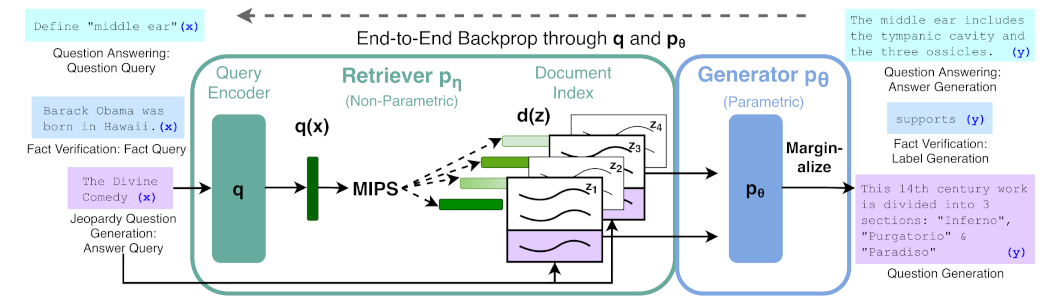
\includegraphics[width=.9\textwidth]{rag-example.png}
	\caption{An overview of the RAG approach, combining a pre-trained retriever with a pre-trained model. From ``Retrieval-Augmented Generation for Knowledge-Intensive NLP tasks'' \citep{rag}}
	\label{rag_overview}
\end{figure}

RAG can be effective in preventing hallucinations by incorporating relevant external information into the generation process, ensuring that responses are more grounded in factual data from a knowledge base.
However, this method is not perfect even after adding contextual data to the query the model could generate a response using its learned parametric memory while ignoring the data retriever by the RAG model.

\subsection{Knowledge Grounding on Queries with Added Context}

Knowledge grounding is the process by which a large language model incorporates external knowledge into its output generation.
In the context of queries with context provided by RAG, a well-grounded model would ensue that answers are consistent with the knowledge in the index rather than in the model's inherent knowledge if they are contradictory.

Various attempts have been made at understanding how good the knowledge grounding of a RAG system is, and on what is the optimal configuration of RAG.

In ``RAGGED: Towards Informed Design of Retrieval Augmented Systems'' \citep{ragged}, the authors create a framework to evaluate these systems and find that different models suit substantially varied RAG setups.
In particular, the performance of the models decreases strongly in Decoder-only models such as Llama when the context passages provides more context, while Seq2Seq models such as Flan-T5 have better performance.

``Characterizing Mechanisms for Factual Recall in Language Models'' \citep{factual_recall}, which is one of the main sources for this thesis, finds that when there is disagreement between the model's knowledge and the provided context then the architecture and size of the large language model will affect the probability of the model choosing to use the context (which is much less prone to hallucinating) as an answer rather than its parametric knowledge.

This paper also introduces a novel way to test this hypothesis by creating a dataset with questions and counterfactual context, an example of which is shown in \cref{query_example}.
By adding counterparametric information to the context, this method allows us to understand whether an answer came is parametric (that is, came from the memory of the model) or contextual (that is, came from the provided context).

\begin{lstlisting}[caption={Example of queries used in \citep{factual_recall}. These queries form the basis and inspiration for the dataset creation done in this thesis}, label={query_example},basicstyle=\ttfamily\small,keywordstyle=\rmfamily\bfseries,keywords={country,in,context,city},captionpos=b,frame=single,breaklines=true,xrightmargin=.15\textwidth,xleftmargin=.15\textwidth,float=h]
The capital of {country} is {in context city}
Q: What is the capital of {country}?
A:
\end{lstlisting}
